\section{Introduction}
\label{sec:intro}
  
The goal of this report is to present a focused partial overview of the state of the art in large scale computer vision (CV).  It aims at identifying areas of expertise in CV which are required or expected to be required in e-science projects at the \href{https://www.esciencecenter.nl/}{Netherlands eScience Center (NLeSc)} as well as defining own research line(s) within the eScience Technology and (applied) research Platform \href{https://www.esciencecenter.nl/site/project/estep}{(eStep)} at the NLeSc.

\subsection{Computer vision}

Computer vision is the science and technology of machines that can see. As a scientific discipline, CV is concerned with the theory for building artificial systems that obtain information from images. It is a type of Arificial intelligence and intercepts a broad range of disciplines such as Optics, Robotics, Image Processing and Pattern recognition. 

\subsubsection{Why is it hard?}
A computer vision researcher always faces the problem to explain why automating vision is a very hard problem, while humans solve it with ease (powered by $30\%$ of the cortex). It is also important to explain the limitations of CV to the potential user of a CV system, especially to scientists from other disciplines. The short answer is: because {\bf seeing is not perceiving}. This illustrated by Figure \ref{fig:CV}.
\begin{figure}[H]
\begin{center}
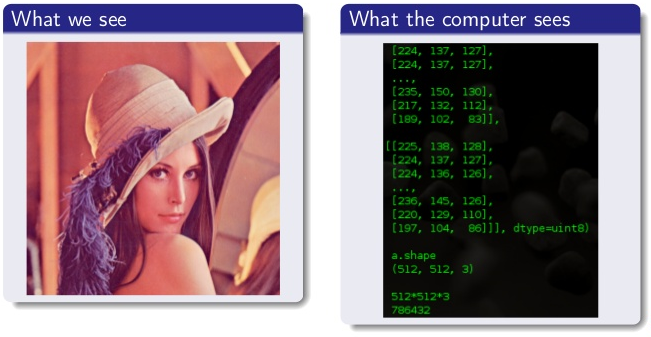
\includegraphics[width=0.8\textwidth]{fig/ManVsPC}
\end{center}
\caption{Human vision vs Computer vision.}
\label{fig:CV}
\end{figure}

Below some factors for deeper understanding of this difficulty are given \cite{Sonka99}:

\begin{enumerate}
\item {\bf Loss of information 3D $\rightarrow$ 2D}. This is a phenomena which occurs in typical image capture device such as camera or a single eye. The corresponding mathematical model is the one of perspective projection- it maps points along rays, but does not preserve angles and collinearity.
\item {\bf Interpretation} of images. Humans use previous knowledge and experience along with the current observation, while a single image is often the only information computer has. This is one of the  main motivation behind using machine learning in CV.
\item {\bf Noise} is inherently present in each measurement in the real world. 
\item {\bf Large data volumes}. This is a main challenge in large scale CV systems.
\item {\bf Brightness measurements} comes by complicated image formation physics. The radiance (brightness, image intensity) depends on irradiance (light source type, intensity and position), observer's position, surface geometry and reflectance properties.
\item {\bf Local window vs. global view.} Usually image analysis algorithms analyze a local part of an image (pixel, neighborhood, region), e.g. the computer sees the image trough e keyhole, which makes it hard to understand the global context.
\end{enumerate}
 
\subsection{Computer vision challenges in other scientific disciplines}
From projects and proposals at NLeSc, where the data for the object of scientific research are captured as 2D/3D images, three main applications of CV can be identified:
\begin{enumerate}
\item {\bf Where is my object? (Localization).} For example, if the object of my study is a freely moving animal, while my camera is fixed somewhere in its habitat, can a CV system find automatically where (potentially) an animal appears on the recorded video, where most frames will probably be of no interest (also, can I keep only the meaningful data?). Technically, the problem is how to automatically find the object of interest or reduce the data to be processed further, so they contain the object of interest (also efficient storage) in large collections of images/videos.
\item {\bf Is my object the same? (Identification).} For example, if I am studying a specific animal, named King Kong, which shares habitat with other animals of the same species, and all the habitat is monitored at different times, can a CV system find me the images where King Kong appears on, as I'm interested only in his movements? Technically, the problem is to (semi-) automatically determine if the study object is the same in multiple instances of photographing it, usually at different time, in different environment and under changing viewing conditions or camera equipment.
\item {\bf What is my object? (Classification).} For example, if King Kong is a gorilla sharing a habitat with other gorillas and chimps, I might like to separate the data of the chimps from those of the gorillas, and even identify new gorillas/chimps captured on camera, as I'm interested in the whole family, friends and enemies of King Kong. Hence, the problem is to (semi-) automatically classify the study object to one of possible categories. Usually the same camera equipment and modality are used to obtain the images/videos.
\end{enumerate}

At NLeSc there have been projects which illustrate these types of questions to be addressed. In the systems biology project \href{https://blog.surf.nl/en/eyr4-blog-5-using-big-data-solutions-to-understand-worm-behavior/}{``Using big data solutions to understand worm behavior''}, the object of research is the {\em C.elegans} worm (see Figure \ref{fig:Celegans}). The source data are high resolution and long videos capturing the behavior of the worm. The first step is to {\em localize} precisely the worm in the large volume of imaging data. 
\begin{figure}[H]
\begin{center}
\includegraphics[width=0.8\textwidth]{fig/Celegans}
\end{center}
\caption{Analysis of behavioral videos of C.elegans.}
\label{fig:Celegans}
\end{figure}
This is a good example of how the object of interest is often studied in controlled environment and one can assume that the most prominent ({\em salient}) object captured on images/videos is the object of interest. In this case, the lab plate ensures relatively uniform background where one can easily find the object of interest in foreground, the worm. The challenge is to find it automatically and to process efficiently large amounts of data.

The localization problem is often related to the {\em segmentation} problem, which is most challenging in the medical imaging domain. Illustration of the difficulty can be seen in Figures \ref{fig:hippo} and \ref{fig:oct}. There is little perceptual difference between the hippocampus and the surrounding brain tissue as well as between some of the retina layers, making it difficult to distinguish even for the human eye.

\begin{figure}[H]
\begin{center}
\includegraphics[width=0.8\textwidth]{fig/hippo}
\end{center}
\caption{Hippocampus segmentation from a brain MRI subvolume. \href{https://www.esciencecenter.nl/project/biomarker-boosting}{BiomarkerBoosting project.}}
\label{fig:hippo}
\end{figure}


\begin{figure}[H]
\begin{center}
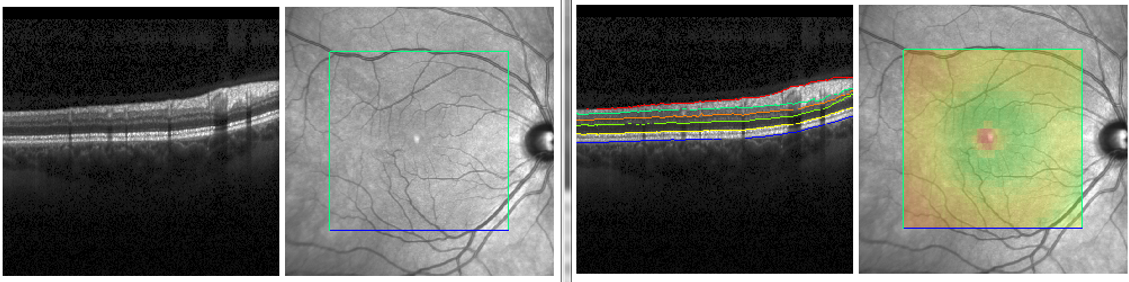
\includegraphics[width=0.8\textwidth]{fig/oct}
\end{center}
\caption{Optical Coherence Tomography (OCT) of retina layers segmentation: image data (left), image segmentation \& retina thickness map (right). \href{https://blog.surf.nl/eyr4-blog-7-lightpath-optical-coherence-tomography-oct-imaging/}{EYR4 project: Light-path for OCT imaging.}}
\label{fig:oct}
\end{figure}

Because of the complexity of the problem, the large number of imaging modalities, equipment and even image formats, usually specific algorithms are developed to segment different body organs and tissues. Since specific solutions are required, which are hard to generalize for other structures, modalities, even less across scientific domains, the image segmentation is left out of the scope of this report.


An example of the {\em identification} problem, is the individual photo-identification of wildlife. This is illustrated on Figure \ref{fig:photoid}. Many species are individually recognizable by characteristic patterns or shape, i.e. by their phenotype.


\begin{figure}[H]
\begin{center}
\includegraphics[width=0.8\textwidth]{fig/photoid}
\end{center}
\caption{Example species with sufficient spot pattering what could be useful for automated photo-identification: (a) whale shark (with reference area),
(b) spotted  tree frog, (c) northern quill, (d) Amazon spotted frog, (e) striped blue crow and (f) mangrove snake.}
\label{fig:photoid}
\end{figure}

An example of the {\em classification} problem is shown on Figure \ref{fig:woodphotoid}. The question is to identify the tree species from microscopic images of wood samples. The {\em Acer} has a different appearance than {\em Toona}, but also within the family there are many species of {\em Toona} which differ- for example {\em Toona ciliata} differs subtly from {\em Toona sinesis} (Figure \ref{fig:treeid}), hence the classification problem could be hierarchical and increasingly difficult.

\begin{figure}[H]
\begin{center}
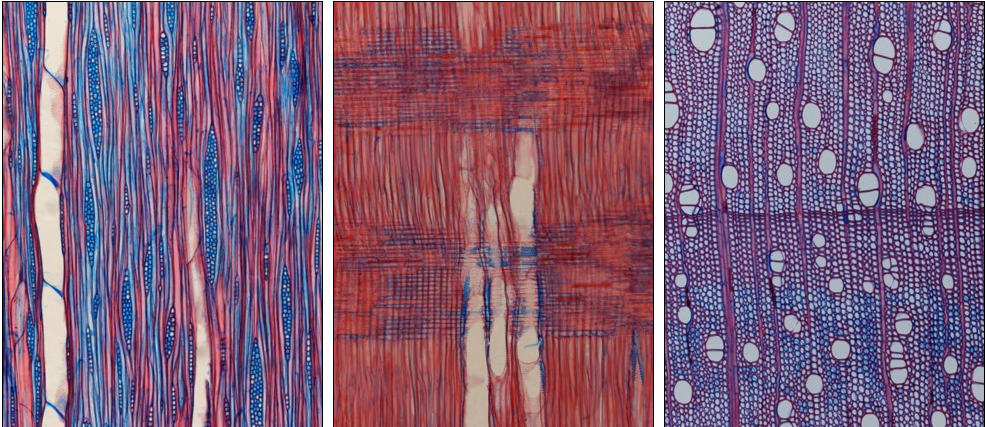
\includegraphics[width=0.8\textwidth]{fig/woodphotoid}
\end{center}
\caption{Left to right: tangential, radial and cross (transversal) sections of stained wood Acer.}
\label{fig:woodphotoid}
\end{figure}

\begin{figure}[H]
\begin{center}
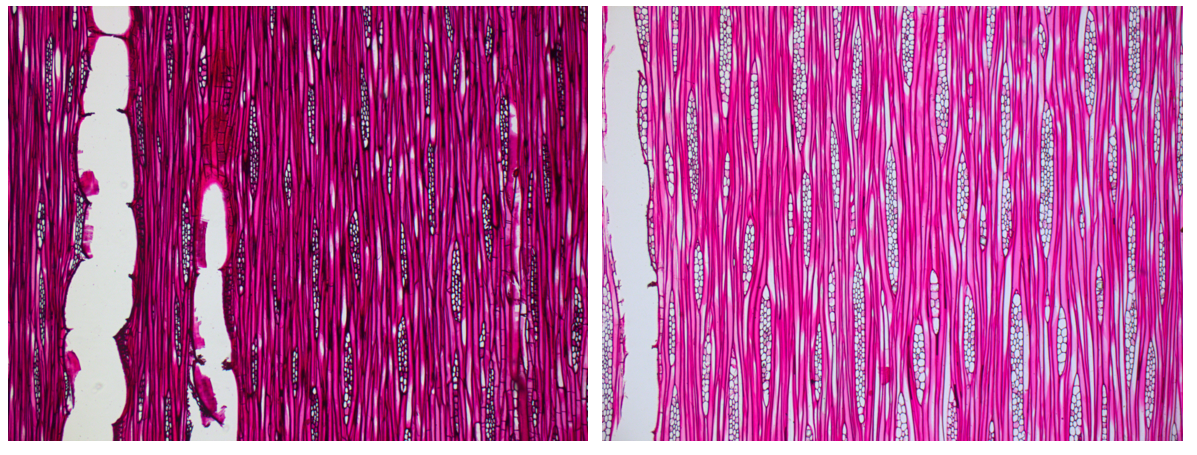
\includegraphics[width=0.8\textwidth]{fig/treeid}
\end{center}
\caption{Tangential section of stained wood. Left: Toona ciliata, Right: Toona sinesis.}
\label{fig:treeid}
\end{figure}

\subsection{Computer vision topics} 
To address the related scientific challenges, three  CV research questions can be defined:
\begin{enumerate}
\item {\bf Visual salience:} How can the CV system determine automatically the most visual salient region(s) in an image?\label{item:sal}
\item {\bf Object/scene identification:} How can the CV system automatically determine whether two images, potentially taken with different cameras under different viewing conditions and transformations, represent the same object/scene?\label{item:ident}
\item {\bf Object/scene detection/classification:} How can the computer recognize automatically to what visual category the object/scene captured in an image belongs to? \label{item:und}
\end{enumerate}

\subsubsection{Other applications}
There are also numerous non-scientific applications related to the above research questions.  For example {\em visual saliency} (\ref{item:sal}) in important in tasks such as:
\begin{itemize}
\item Automatic target detection (see Fig. \ref{fig:sal})
\item Robot navigation using salient objects
\item Image and video compression
\item Automatic cropping/centering images for display on small portable screens, etc.
\end{itemize}

\begin{figure}[H]
\begin{center}
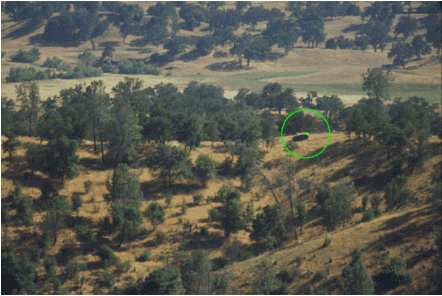
\includegraphics[width=0.8\textwidth]{fig/saliency}
\end{center}
\caption{Example of a saliency model detecting the vehicle as being the most salient object in a complex scene.}
\label{fig:sal}
\end{figure}

Few of the numerous applications related to {\em object/scene identification} (\ref{item:ident}) are:
\begin{itemize}
\item Stereo and wide-baseline matching
\item Image panorama stitching/creation
\item Automatic reconstruction of 3D scenes, etc.
\end{itemize}

Automatically understating the {\em semantics of an object/scene} (\ref{item:und}) in the form of image classification, have many applications like:
\begin{itemize}
\item Image search engines
\item Organizing photo collections
\item Autonomous driving
\item Human machine interaction
\item Digital forensic investigation, etc.
\end{itemize}

This is a complex and high-level computer vision task, with the goal of making machines see like humans and be able to infer both general principles as well as current situations from images. Example of a trained system for scene categorization is shown on Fig.\ref{fig:mitdemo}.
\begin{figure}[H]
\begin{center}
\includegraphics[width=0.8\textwidth]{fig/mitdemo}
\end{center}
\caption{ \href{http://places.csail.mit.edu/demo.html}{MIT Scene Recognition Demo.}}
\label{fig:mitdemo}
\end{figure}

In fact, the majority of CV researchers traditionally work on non-scientific applications, focusing on the third and most challenging problem. Addressing the problems faced by other domain scientist, while still conducting generic and widely applicable computer vision research, seems to fit best the strategy of NLeSc and eStep. 

The overview is by no means complete, it rather tries to summarize the research in the field along the above three questions in the last years. The report is structured along the main outputs of the CV research, namely, scientific publications in Section \ref{sec:pubs}, software in Section \ref{sec:soft} and datasets in Section \ref{sec:db}. Some potential scientific applications are shown in Section \ref{sec:app}. The conclusions and recommendations are given is section \ref{sec:conc}.